\chapter{Technische Umsetzung}
\section{Beschreibung der App}
\subsection{Funktionen der jeweiligen Seiten}
\subsubsection{Homepage}
Die Homepage der App zeigt ein zufälliges und derzeit besonders beliebtes Spiel an, welches von der BoardGameGeek \ac{API} bezogen wird.
Die Generierung erfolgt automatisch und bei jedem Aufruf der Seite neu. Daher wird dieser Fähigkeit in der \texttt{ngOnInit()}-Funktion auf der Homepage aufgerufen.
Darüber hinaus dient die Homepage primär als Ausgangspunkt für die Navigation zu den anderen Seiten (siehe Tab. \ref{tab:homepage}).
\begin{table}[H]
    \centering
    \begin{tabular}{|c|c|}
        \hline
        \textbf{Funktion} & \textbf{Beschreibung} \\
        \hline
        \texttt{goToSearch()} & Navigiere zur Suchleiste. \\
        \texttt{goToWishlist()} & Navigiere zur Wunschliste. \\
        \texttt{goToInventory()} & Navigiere zum Inventar. \\
        \texttt{openGameDetails()} & Navigiere zur Infopage des zufälligen Spiels. \\
        \hline
    \end{tabular}
    \caption{Funktionen der Homepage.}
    \label{tab:homepage}
\end{table}

\subsubsection{Searchpage}
\subsubsection{Infopage}
\subsection{Genutzte Interfaces und Modelle}
In der Welt der Softwareentwicklung ist es entscheidend, dass Daten, die zwischen verschiedenen
Systemen ausgetauscht werden, klar definierte Strukturen haben. TypeScript-Interfaces sind hierbei
äußerst nützlich, insbesondere wenn es um die Interaktion mit APIs geht.
Das Boardgame Interface beschreibt alle wesentlichen Informationen eines Brettspiels, die über die
BGG-API abgerufen werden und in einer MongoDB gespeichert werden. Dazu gehören Details wie der
eindeutige Identifikator des Spiels, das Veröffentlichungsjahr, die Spieleranzahl, die Spieldauer, das
empfohlene Alter, eine Beschreibung und ein Vorschaubild. Dieses Interface stellt sicher, dass die von
der API gelieferten Daten vollständig und in einer korrekten Form sind, die direkt in der Datenbank
gespeichert werden kann (so dass auch Falls kein Bild in der Api Verfügbar ist dies abgespeichert
wird).
Das Game Interface hingegen ist eine reduzierte Version des Boardgame Interfaces. Es kann in
Situationen eingesetzt werden, in denen nicht alle Informationen eines Brettspiels benötigt werden,
wie zum Beispiel in einer Übersichtsliste von Spielen. Durch das Weglassen von Details wie Spielzeit
oder Altersangabe wird die übertragene Datenmenge verringert, was die Effizienz verbessern und die
Ladezeiten verkürzen kann.
Das Randomgame Interface ist spezialisiert auf die Darstellung eines zufällig ausgewählten Spiels aus
den Top 50 der am besten bewerteten Brettspiele. Neben der Standardinformation wie Identifikator,
Name, Veröffentlichungsjahr und einem Bild des Spiels, speichert dieses Interface zusätzlich den Rang
des Spiels, also seine Position in der Rangliste. Diese Information ist besonders wertvoll, um auf einen
Blick die Beliebtheit eines Spiels einschätzen zu können, diese wird basierend auf ihrer Position in der
Top 50 eingelesen.
Diese Interfaces sind essenzielle Bausteine für die zuverlässige Datenarchitektur. Sie sorgen nicht nur
für eine korrekte Typisierung und eine klare Vertragsgestaltung zwischen dem Backend (der API) und
dem Frontend, sondern tragen auch dazu bei, den Datenfluss übersichtlich und wartbar zu halten. So
kann die Software sich an verändernde Anforderungen anpassen, ohne dass es zu einem
Durcheinander in der Datenstruktur kommt.

\subsubsection{Boardgame}
Das \texttt{Boardgame} Interface repräsentiert die Struktur zur Speicherung von Informationen über ein
Brettspiel. Die Eigenschaften sind wie folgt:
\begin{table}[H]
    \centering
    \begin{tabular}{|c|c|c|}
        \hline
        \textbf{Eigenschaft} & \textbf{Typ} & \textbf{Beschreibung} \\
        \hline
        \texttt{objectId} & \texttt{string} & Dient der eindeutigen Identifikation eines Spiels. \\
        \texttt{yearPublished} & \texttt{string} & Das Jahr, in dem das Spiel veröffentlicht wurde. \\
        \texttt{minPlayers} & \texttt{string} & Die minimal erforderliche Anzahl an Spielern. \\
        \texttt{maxPlayers} & \texttt{string} & Die maximal mögliche Anzahl an Spielern. \\
        \texttt{playingTime} & \texttt{string} & Die durchschnittliche Spieldauer. \\
        \texttt{minPlayTime} & \texttt{string} & Die minimal mögliche Spieldauer. \\
        \texttt{maxPlayTime} & \texttt{string} & Die maximal mögliche Spieldauer. \\
        \texttt{age} & \texttt{string} & Die empfohlene Altersangabe. \\
        \texttt{description} & \texttt{string} & Eine Beschreibung des Spiels. \\
        \texttt{name} & \texttt{string[]} & Eine Liste von Namen, unter denen das Spiel bekannt ist. \\
        \texttt{publisher} & \texttt{string[]} & Eine Liste von Verlagen, die das Spiel veröffentlicht haben. \\
        \texttt{averageWeight} & \texttt{string} & Die durchschnittliche Komplexität des Spiels. \\
        \texttt{averageRating} & \texttt{string} & Die durchschnittliche Bewertung des Spiels. \\
        \texttt{thumbnail} & \texttt{string} & Ein Link zu einem Vorschaubild des Spiels. \\
        \texttt{usersRated} & \texttt{string} & Die Anzahl der Benutzer, die das Spiel bewertet haben. \\
        \hline
    \end{tabular}
    \caption{Eigenschaften des \texttt{Boardgame} Interfaces.}
    \label{tab:boardgame}
\end{table}

\subsubsection{Game}
Das \texttt{Game} Interface repräsentiert eine reduzierte Version des \texttt{Boardgame} Interfaces. Es
wird verwendet, um die Datenmenge zu verringern, wenn nicht alle Informationen eines Spiels
benötigt werden. Die Eigenschaften sind hierbei wie folgt:
\begin{table}[H]
    \centering
    \begin{tabular}{|c|c|c|}
        \hline
        \textbf{Eigenschaft} & \textbf{Typ} & \textbf{Beschreibung} \\
        \hline
        \texttt{objectId} & \texttt{string} & Dient der eindeutigen Identifikation eines Spiels. \\
        \texttt{name} & \texttt{string} & Gibt den Namen des Spiels an. \\
        \texttt{yearPublished} & \texttt{string} & Das Jahr, in dem das Spiel veröffentlicht wurde. \\
        \texttt{thumbnail} & \texttt{string} & Ein Link zu einem Vorschaubild des Spiels. \\
        \hline
    \end{tabular}
    \caption{Eigenschaften des \texttt{Game} Interfaces.}
    \label{tab:game}
\end{table}
\textbf{Hinweis:} Es gibt zwei Versionen des \texttt{Game} Interfaces, eine mit der Eigenschaft „thumbnail“ und eine
ohne. Es ist wichtig sicherzustellen, dass die richtige Version verwendet wird, um der erforderlichen
Datenstruktur für die Anwendung zu entsprechen.

\subsubsection{Randomtopgame}
Das \texttt{Randomtopgame} Interface repräsentiert die Struktur zur Speicherung von Informationen über ein
zufällig ausgewähltes Spiel aus den Top 50 der am besten bewerteten Brettspiele. Hierfür werden folgende
Eigenschaften definiert:
\begin{table}[H]
    \centering
    \begin{tabular}{|c|c|c|}
        \hline
        \textbf{Eigenschaft} & \textbf{Typ} & \textbf{Beschreibung} \\
        \hline
        \texttt{id} & \texttt{string} & Dient der eindeutigen Identifikation eines Spiels. \\
        \texttt{name} & \texttt{string} & Der Name des Spiels. \\
        \texttt{yearPublished} & \texttt{string} & Das Jahr, in dem das Spiel veröffentlicht wurde. \\
        \texttt{thumbnail} & \texttt{string} & Ein Link zu einem Vorschaubild des Spiels. \\
        \texttt{rank} & \texttt{string} & Die Position des Spiels in der Rangliste. \\
        \hline
    \end{tabular}
    \caption{Eigenschaften des \texttt{Randomtopgame} Interfaces.}
    \label{tab:randomtopgame}
\end{table}
\section{Beschreibung der verwendeten Services}


\section{Beschreibung der verwendeten APIs}
\subsection{BoardGameGeek XML API }

Die BoardGameGeek XML API bietet eine Schnittstelle zum Zugriff auf eine Vielzahl von Informationen rund um Brettspiele,
die auf BoardGameGeek.com, einer umfangreichen Datenbank und Community für Brettspiel-Enthusiasten,
verfügbar sind. Diese API ermöglicht es Entwicklern druch verschiedene Endpoints auf Spielinformationen,
Benutzerkollektionen und Forendiskussionen zuzugreifen. Dabei zu beachten ist, dass die API die Antwort als XML-Format weitergibt. 
Da häufig mit JSON gearbeitet wird ist eine mögliche Umformung der Daten sinnvoll.

\large Suchfunktion

Eine der drei benutzten Endpunkte ist die `/xmlapi/search`-Funktion bei der Nutzer als Input einem spezifischen Suchterm eingeben.
Als Ergebnis enthält man eine Liste an Brettspielen in XML Format, deren Namen oder Alias im Suchbegriff enthalten war.
Die Suchfunktion Antwort enthält folgende Informationen:
\begin{itemize}
    \item {objectId des Brettspiels}
    \item {Name des Brettspiels}
    \item {Erscheinungsjahr des Brettspiels}
\end{itemize}

Die reale Ausgabe für den fiktiven Suchterm ``Frika'' würde somit folgendes zurückgeben: 
\begin{figure}[h]
    \centering
    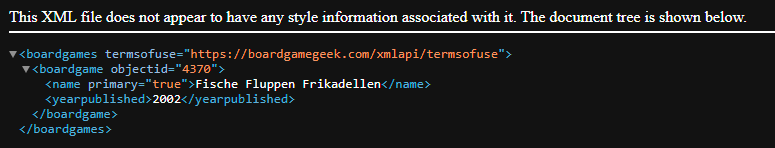
\includegraphics[width=1\textwidth]{graphics/Search_API.png}
    \caption{Ergebnis der `/xmlapi/search`-Funktion bei Suchterm Frika}
    \label{fig:Search_API}
\end{figure}

 \large Detaillierte Spielinformationen

Der zweite Endpunkt ist die `/xmlapi/boardgame/<gameid>`-Funktion und dient dazu,
detaillierte Informationen zu einem Brettspiel zu erhalten. Nutzer könnten hier noch einige weitere Parameter mitgeben um spezifische Informationen zu erhalten, jedoch ist dies in unserem Projekt nicht notwendig, da die Ergebnisse schon detailliert genug sind.
Die gameId ist hierbei der Input, ist gleichzusetzen mit der objectId und kann aus des oben erhaltenen Ergebnisses der Suchfunktion entnommen werden.
Die detaillierten Spielinformationen enthalten folgende Informationen:

\begin{table}[H]
    \centering
    \begin{tabular}{|c|c|}
        \hline
        \textbf{Name} & \textbf{Formattyp} \\
        \hline
        \texttt{objectId} & \texttt{String} \\
        \texttt{yearPublished} & \texttt{String} \\
        \texttt{minPlayers} & \texttt{String} \\
        \texttt{maxPlayers} & \texttt{String} \\
        \texttt{playingTime} & \texttt{String} \\
        \texttt{minPlayTime} & \texttt{String} \\
        \texttt{maxPlayTime} & \texttt{String} \\
        \texttt{age} & \texttt{String} \\
        \texttt{description} & \texttt{String} \\
        \texttt{name} & \texttt{Array (String)} \\
        \texttt{publisher} & \texttt{Array (String)} \\
        \texttt{averageWeight} & \texttt{String} \\
        \texttt{averageRating} & \texttt{String} \\
        \texttt{thumbnail} & \texttt{String (URL to thumbnail image)} \\
        \texttt{usersRated} & \texttt{String} \\
        \hline
    \end{tabular}
    \caption{Die zurückgegebenen detaillierten Informationen}
    \label{tab:boardgame_properties}
\end{table}

Es ist zu erkennen, dass der Name und der Publisher Arrays sind. Dies lässt sich darauf zurückführen, dass es mehrere Namen für dasselbe Spiel gibt (teilweise auch in anderen Sprachen) und mehrere Entwicklet beteiligt sein können.

\large Game of the Day

Der dritte Endpunkt im Bunde ist die `xmlapi2/hotoverall`-Funktion. Sie gibt die top 50 Spiele mit besonders guter Bewertung und Beliebtheit zurück.
Dabei werden genau fünf unterschiedliche Informationen aufgeführt:
\setlength{\itemsep}{-1pt}
\setlength{\parskip}{-1pt}
\begin{itemize}
    \item id: String (objectId von vorher earlier)
    \item rank: String (Ranking Position der Top 50 Spiele)
    \item thumbnail: String (URL to thumbnail image)
    \item name:  String        
    \item yearpublished 
\end{itemize}

Im Anschluss kann ebenfalls mit der ObjectId eine Anfrage für detaillierte Informationen gestartet werden. 
Einsatz findet dieses Verfahren wenn mit einem Klick das Game of the Day ausgewählt wird und somit die zurückgegebene ObjectId auf die Infopage
weitergeleitet wird. Somit konnte eine weitere Seite wiederverwendet werden und zudem ein neues Feature für die App ermöglicht. 

\subsection{MongoDB API}

In diesem Teil wird nur der externe Aufruf auf den selbsterstellten MongoDB API-Endpunkt behandelt. 
Der Interne Aufbau der MongoDB wird in der Beschreibung der App aufgeführt. Es gibt insgesamt drei Zugriffsmethoden für jede Collection auf die MongoDB: 
searchGamesWishlist(), searchGamesInventory(), addToWishlist(gameData), addToInventory(gameData), removeFromWishlist(objectId), removeFromInventory(objectId)\bigskip


Die Get Methode, hier searchGames..., bezieht sich af den HTTP Endpoint 

``http://localhost:8999/wishlisht'' oder beziehungsweise ``\ldots/inventory'' und liefert eine Liste aus JSON-Elementen zurück.
Für das hinzufügen von Brettspielen wird die HTTPClient Methode POST benutzt und die gameData übergeben, wobei Gamedata ein Objekt des Modells Boardgame.ts ist. 
Dieses Objekt wird dann in eine JSON Form in die ausgewählte collection hinzugefügt. Bei der Entfernung eines Spiels wird als Parameter die ObjectId des Spiels übergeben.
Dieser einzigartige Klassifikator sorgt dafür, dass wenn ein Spiel in der Collection enthalten ist, dass diese ObjectId als Klassifikator verwendet, wird dieses Brettspiel entfernt.
Des Weiteren ist dies aus Effizienz gründen vorteilhaft, da kein komplettes Objekt übergeben wird, geparsed werden muss und schlussendlich verglichen. Es kann direkt eine Überprüfung statt finden.


\begin{center}
    \begin{lstlisting}[caption={Löschaufruf der MongoDB API}, label=lst:jscode]
    this.http.delete(`${this.inventoryUrl}/${objectId}`)
\end{lstlisting}
\end{center}


\subsection{Verwendung der APIs im Projekt selbst}

Die Definition der Methoden zum aufrufen der API-Endpunkte ist in dem   File ``board-game.service.ts'' des ``services''-Ordner zu finden.
Dazu wird das HTTPClient Modul importiert und es wird ein htttp.get Aufruf mit den jeweiligen Parametern durchgeführt. Da das Ergebnis in Form einer XML-Datei vorliegt und es vorteilhafter ist mit einem JSON-Format zu arbeiten wird zu Beginn eine Transfarmation des Formats in die JSON Form durchgeführt.
Dies geschieht konkret durch das importierte Modul ``xml2json''. \bigskip 

Die daraufhin vorliegende JSON kann nun dem Modell game.ts, boardgame.ts oder randomtopgame.ts zugewiesen werden. Also eine initialisierung einer Liste von Objekte dieser Modelle basierend auf dem spezifischen API-Aufruf.
Im folgenden wird dann Array als return Element der Funktion definiert. Dies ermöglicht es erstmalig ein subscribe auf die Funktion zu legen und auf der benötigten Page anzuzeigen. \bigskip 

Die konkrete Verwendung der APIs ist auf den folgenden Pages ist wiefolgt:

\begin{itemize}
    \setlength{\itemsep}{-1pt}
    \setlength{\parskip}{-1pt}
    \item Homepage
        \begin{itemize}
        \item Game of the Day mit `xmlapi2/hotoverall`-Funktion
        \end{itemize}
    \item Searchpage
        \begin{itemize}
        \item Suchfunktion mit `/xmlapi/search`-Funktion
        \end{itemize}
    \item Inventory, Wishlist
        \begin{itemize}
        \item MongoDB GET mit ``http://localhost:8999/inventory/''-Funktion 
        \end{itemize}
    \item Infopage
    \begin{itemize}
    \item Detaillierte Spielinformationen mit `/xmlapi/boardgame/<gameid>`-Funktion 
    \item MongoDB mit ``http://localhost:8999/inventory?objectId''-DELETE Funktion
    \item MongoDB mit ``http://localhost:8999/inventory?gameData''-ADD Funktion
    \item MongoDB mit ``http://localhost:8999/wishlisht?objectId''-DELETE Funktion
    \item MongoDB mit ``http://localhost:8999/wishlisht?gameData''-ADD Funktion
    \end{itemize}

\end{itemize}

\section{Anleitung zum Starten der Applikation}
